\documentclass{article}
\usepackage[a4paper,left=2.5cm,right=2.5cm,top=2.5cm,bottom=2.5cm]{geometry}
\usepackage[utf8]{inputenc}
\usepackage{titlesec}
\usepackage{hyperref}
\usepackage{enumitem}
\usepackage{graphicx}
\usepackage{array}
\usepackage{hhline}

\titleformat{\section}
{\normalfont\Large\bfseries}{Unit~\thesection}{1em}{}
\graphicspath{ {images/} }

\begin{document}

\begin{center}
	{\Large CIS*2520 Mock Exam (Summer 2017)} \\
	\smallskip
	All questions are used from Courselink via \url{https://courselink.uoguelph.ca/d2l/le/content/470592/Home}.
\end{center}

\medskip
\section{Lists, Stacks and Queues}

\begin{enumerate}
	\item Define the following with respect to software design:
		\begin{enumerate}[label=\alph*.]
			\item Modularity \\\\
			\item Reuse \\\\
			\item Maintainability \\\\
			\item Coupling \\\\
			\item Cohesion \\\\
		\end{enumerate}
	\item Define Test-Driven Development. \\\\
	\item List ten different programming languages as well as their level of abstraction (Moderate, High, Very High).
		\begin{enumerate}[label=\arabic*.]
			\item \rule{8cm}{0.1mm}
			\item \rule{8cm}{0.1mm}
			\item \rule{8cm}{0.1mm}
			\item \rule{8cm}{0.1mm}
			\item \rule{8cm}{0.1mm}
			\item \rule{8cm}{0.1mm}
			\item \rule{8cm}{0.1mm}
			\item \rule{8cm}{0.1mm}
			\item \rule{8cm}{0.1mm}
			\item \rule{8cm}{0.1mm} \\
		\end{enumerate}
	\item Write pseudocode for a multiply and a subtract operation for the fraction ADT. What does the integer portion of the Fraction struct represent? List any additional operation(s) that would be required in order to make use of that part of the struct. (Fraction ADT available on Courselink)
	\newpage
	\item Write the following three algorithms:
		\begin{enumerate}[label=\arabic*.]
			\item The algorithm for the addToLocation() operation for the List ADT. This operation should add an element to the list at a specific location in the list (identified by a number). Use the same specification format as has been used to describe operations in this lesson. Include all necessary parameters and return values in the signature of your specification. Be sure to include preconditions and postconditions.
			\vspace{3cm}
			\item The algorithm to delete a node from the nth position of a linked list. The operation should return the deleted data and ensure that the remaining elements of the list are properly connected.
			\vspace{3cm}
			\item The algorithm for inserting a node in sorted order given an array implementation of a list. The algorithm should take the data as a parameter.
			\vspace{3cm}
		\end{enumerate}
	\item Would a double linked list or a single linked list be a better choice for encapsulation in a Stack ADT? Justify your opinion.
		\vspace{3cm}
	\item Write the algorithms for push() and pop() given an array implementation of a stack. Show the stack struct definition as well.
		\vspace{4cm}
	\newpage
	\item Create a design or prototype of a reverse polish calculator program. You should limit operations to + - * and /. Use a stack ADT in your design.
	\newpage
	\item What is the Computation complexity of the enqueue() and dequeue() operations expressed in Big O notation? \\\\
	\item What additional information must be kept track of in order to use a conventional array as a circular buffer? Give the Queue struct that you would use if you were writing a circular buffer queue implementation.
	\vspace{4cm}
	\item Write the algorithm for dequeuing an item from a circular buffer queue.
	\vspace{4cm}
	\item Which of the following statements about queues is untrue?
		\begin{enumerate}[label=\alph*.]
			\item Queues can have elements inserted at any position in the data structure.
			\item The first element inserted into a queue will be the first element taken out of the queue.
			\item Queues can be found in the real world.
			\item The size of a queue data structure is bounded only by the size of the computer memory.
			\item A queue is somewhat similar to a stack.
		\end{enumerate}
	\item Which List operation would be most likely to be the one encapsulated if you were writing a remove operation for a queue?
		\begin{enumerate}[label=\alph*.]
			\item addHead(elementToBeAdded)
			\item length()
			\item removeBack()
			\item removeHead()
			\item insert(position, elementToBeAdded)
		\end{enumerate}
	\item Given the following queue: A B b E r S T, where A is the front of the queue, what will the queue content be after two remove operations?
		\begin{enumerate}[label=\alph*.]
			\item A B b E r S T
			\item b E r S T
			\item A B b E r S
			\item T A B b E r
			\item The queue will be empty.
		\end{enumerate}
	\newpage
	\item Given the following queue: t y 5 8 i 2 d t e, what should a call to length() return?
		\begin{enumerate}[label=\alph*.]
			\item 9
			\item 8
			\item 10
			\item It will generate an error because of the mixed data types.
			\item 3
		\end{enumerate}
\end{enumerate}

\medskip
\section{Hash Table and Binary Trees}

\begin{enumerate}
	\item If you were implementing a student record system for a small music school with fewer than 200 students, and were using associative arrays as the data structure, how would you implement your associative array? Would you make a different choice if your student record system was for a university?
	\vspace{2cm}
	\item Write a ’to-do list’ of the things you would need to do (including research and learning) in order to implement the borrowers’ library example. Try to make the list very specific. Use the to-do list to estimate the amount of time it would take you to implement and test the application (round up to the nearest hour).
	\vspace{5cm}
	\item Using the division method, calculate hash values for the following set of keys:
		\begin{center}	
			\(\{54, 77, 82, 13, 991, 308, 68, 45, 1001, 73\}\)
		\end{center}
		Calculate once using a table size of 11. Calculate a second time using a table size of 12. Do you notice anything about the distributions of the calculated values?
		\vspace{2cm}
	\newpage
	\item The expected search time for Linear probing can be calculated by the following formula:
		\begin{enumerate}[label=\roman*.]
			\item \(O(1 + {1 \over 1 - loadFactor})\) for a successful search.
			\item \(O(1 + {1 \over {(1 - loadFactor})^2})\) for an unsuccessful search.
		\end{enumerate}
		Create a chart showing the expected search times (successful and unsuccessful) for the following load factors: .10, .20., .30, .40, .50, .60, .70, .80, .85, .90, .95. \\
		What do these numbers tell you?
	\vspace{2cm}
	\item Suppose you have two hash functions H1 and H2 where H1(87) = 10, H2(87) = 3 and H1(42)=10, H2(42)=7. Further suppose that the key 87 is inserted into the table first and then the key of 42. Show the sequence of table positions tried when using random probing with a constant of 37 and a table size of 11.
	\vspace{4cm}
	\item The expected time for a search using Double hashing can be calculated by the following formula:
		\begin{enumerate}[label=\roman*.]
			\item \(O({1 \over loadFactor} \times (1 + ln({1 \over {1 - loadFactr}})))\) for a successful search.
			\item \(O({ 1 \over {1 - loadFactor}})\) for an unsuccessful search.
		\end{enumerate}
		Create a chart showing the expected search times (successful and unsuccessful) for the following load factors: .10, .20., .30, .40, .50, .60, .70, .80, .85, .90, .95. \\
		What do these numbers tell you?
	\vspace{2cm}
	\item The loadFactor of a hash table using separate chaining to resolve collisions is calculated as the number of \textbf{keys / the number of chains}. The expected length of search, successful or unsuccessful, of Separate Chaining is \(O(1 + loadFactor)\).
		\begin{enumerate}[label=\alph*.]
			\item Calculate a chart of the predicted search times for the following load factors: .10, .20., .30, .40, .50, .60, .70, .80, .85, .90, .95.
			\vspace{2cm}
			\item What do these numbers tell you?
			\newpage
			\item What factors would you consider when selecting a collision resolution approach for a hash table?
			\vspace{2cm}
		\end{enumerate}
	\item The order that nodes are inserted into a tree can greatly affect the structure of the tree. Draw the binary tree that is constructed by adding the seven names in the following order:
		\begin{enumerate}[label=\arabic*.]
			\item Sleepy
			\item Bashful
			\item Doc
			\item Dopey
			\item Sneezy
			\item Happy
			\item Grumpy
		\end{enumerate}
	\vspace{1.5cm}
	\item Trace the algorithms for level-order traversal using a hand drawn tree. What order are the nodes of the tree printed in? Can you tweak the algorithm to reverse the order?
	\vspace{6cm}
	\item One of the most frequent uses of a binary tree is as a search tree. The object is to search through the data to find out if a particular element is part of the data. Write a recursive find procedure for a binary tree. Start with the root node of the tree. Your procedure can be in \(C\) or in pseudocode. Be sure to pass in the compare function pointer.
	\vspace{6cm}
	\item Give the in-order traversal and the pre-order traversal of the tree shown below.
		\begin{center}
			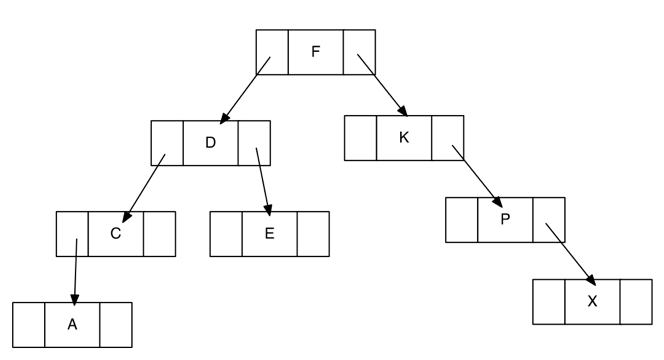
\includegraphics[scale=0.5]{alphatree}
		\end{center}
	\vspace{2cm}
	\item Write the pseudocode or \(C\) code for a compare operator. A compare operator must return three distinct values, one for when the first parameter is larger, one for when the second parameter is larger, and one for when the two parameters are equal. The convention is to use 1, 0, and -1 for the three values. Zero for equal values, 1 for the first string being larger, -1 for the second.
	\vspace{5cm}
	\item The delete operation relies on a recursive function to find the minimum value in a subtree. The minimum value will always be the leftmost leaf of the subtree. Write the findMinimum function (in pseudocode or in \(C\)).
	\vspace{5cm}
	\newpage
\end{enumerate}

\medskip
\section{Heaps and Priority Queues}

\begin{enumerate}
	\item Develop a formula to calculate the position of a parent node in an array-implementation of a heap. The only input information to the formula is the position of the current node.
	\vspace{3cm}
	\item Create the \(C\) struct for a binary-tree based heap. Your struct should have members for the heap, the last added element, the next position, and function pointers to manipulate void* data.
	\vspace{4cm}
	\item Heaps do not have to be a min/max binary tree. Many variations of heaps are possible. Use internet resources to learn about one of the following different types of heaps: skew heaps, binomial heap, or leftist heap. Write the pseudocode for insert and delete operations for the type of heap you chose.
	\vspace{6cm}
	\item The complexity of insert and delete for a binary heap is \(O(log(N))\). Why is that? Create a written explanation, chart, or diagram that explains why \(log(N)\) is the complexity for those operations.
	\vspace{6cm}
	\item Consider the implementation of a priority queue using an array, a linked list, and a heap. For each implementation, provide the pseudocode for the insert and removeMax operation. What is the complexity of those operations in each case?
		\begin{enumerate}[label=\alph*.]
			\item Array Implementation
			\vspace{6cm}
			\item Linked List Implementation
			\vspace{6cm}
			\item Heap Implementation
			\vspace{6cm}
		\end{enumerate}
	\item Use the Internet to find an additional approach to avoiding starvation in a priority queue, other than the two mentioned in the notes. Describe this third approach.
	\vspace{3cm}
	\item Assume you have a computer that can execute 1 billion instructions per second. How long (in seconds / minutes / days / months / years) would that computer take to execute an algorithm of the complexity give for each of the number of data items shown in the table below. \\
		\begin{center}
			\renewcommand{\arraystretch}{1.25}
			\begin{tabular} { | l | l | l | l |}
				\hline
				Algorithm order & 10,000 data items & 1 million data items & 1 billion data items \\
				\hhline{|=|=|=|=|}
				\(O(\log N)\) & & & \\ \hline
				\(O(N)\) & & & \\ \hline
				\(O(N \log N)\) & & & \\ \hline
				\(O(N^{2})\) & & & \\ \hline
				\(O(2^{N})\) & & & \\ \hline
			\end{tabular}
		\end{center}
	\vspace{2mm}
	\item Create a table showing the count of the primitive operations for the algorithm for adding a node to the end of a singly linked list. The algorithm is given in the Linked List materials for this course. What is the big O complexity for that algorithm?
	\vspace{4cm}
	\item Consider the following three algorithms for determining whether anyone in a room of people has the same first name as a target person. What is the worst case scenario for these algorithms? For each algorithm, how many questions will be asked in the worst case? What is the Big O complexity class for each algorithm?
		\begin{enumerate}[label=\arabic*.]
			\item The target person says their name. All the people with the same name stand up.
			\vspace{2cm}
			\item The target person approaches each person in the room to ask them their name. If the person approached has the same name as the target person, the search is successful and stops.
			\vspace{2cm}
			\item The target person asks one person about their name. If person one does not have the same name, the target person asks person one to ask the next person (person two). Person two responds to person one, who tells the target person the answer. If that name doesn’t match, the target person asks person one to tell person two to ask person three. Person three responds to person two who responds to person one who tells the target person. This algorithm continues until the last person has been asked.
			\vspace{2cm}
		\end{enumerate}
	\newpage
	\item Consider the following four functions:
		\begin{itemize}
			\item function 1: \(O(2^N )\)
			\item function 2: \(O(N^{5 / 3})\)
			\item function 3: \(O(N \log N)\)
			\item function 4: \(O(N ^ {\log N})\)
		\end{itemize}
		List the four functions in order of increasing computational complexity:
		\begin{enumerate}[label=\arabic*.]
			\item \rule{4cm}{0.1mm}
			\item \rule{4cm}{0.1mm}
			\item \rule{4cm}{0.1mm}
			\item \rule{4cm}{0.1mm}
		\end{enumerate}
	\item Create a table showing the count of primitive operations for a bubble sort. What is the worst case big O complexity class for a bubble sort?
	\vspace{4cm}
 
\end{enumerate}

\medskip
\section{Balanced Trees and Sorting}

\begin{enumerate}
	\item Using a tree graph, create a binary search tree (BST) by inserting the numbers between 1 and 9 into the tree, in order. What do you notice about the tree? 
		\vspace{5cm} \\
		Using another tree graph, insert the same numbers in the following order 5 3 7 4 2 8 6 9 1. What do you notice about the tree this time?
	\vspace{5cm}
	\item The AVL tree shown in this figure is unbalanced. It needs a right rotation on node 38 to complete the balancing step. 
		\begin{center}
			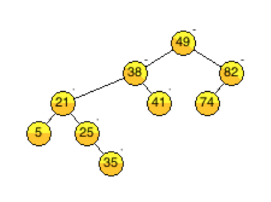
\includegraphics[scale=0.75]{avltree}
		\end{center}
		List the steps required to complete the rotation.
	\vspace{3cm}
	\item Write \(C\) code showing the struct you would implement for a fully abstracted b-tree. 
		\vspace{4cm} \\
		Write the \(C\) code for the insert function for the b-tree.
	\vspace{4cm}
	\item Describe the key similarities and differences between red-black trees and AVL trees.
	\vspace{4cm}
	\item What is the maximum height of an AVL tree with 9 nodes? Assume that an AVL tree with one node is height 1. Can you find a formula for the maximum height of an AVL tree with N nodes?
	\vspace{4cm}
	\item Design an augmented AVL tree which can quickly compute the number of nodes in any tree or subtree. Discuss changes to the struct for the AVL tree as well as necessary changes to any of the algorithms for the ADT.
	\vspace{12cm}
	\item Which of the following statements is true about Insertion Sort?
		\begin{enumerate}[label=\alph*.]
			\item It is a comparison Sort.
			\item It is an adaptive Sort.
			\item It has an \(O(n \log n)\) complexity for the best case.
			\item It has an \(O(n^2 )\) complexity for the worst case.
			\item It performs more comparisons than Selection Sort.
			\item It is always outperformed by divide and conquer sorts.
			\item It requires \(O(1)\) extra memory.
			\item It is an in-place sort.
		\end{enumerate}
	\newpage
	\item Which of the following scenarios might be a good situation in which to use insertion sort?
		\begin{enumerate}[label=\alph*.]
			\item When only alphabetical sort is required.
			\item When you are sorting more than 20 items.
			\item When you are sorting fewer than 20 items.
			\item When you have very little extra memory space.
			\item When you need an extremely fast sort.
			\item When the comparison operator is computationally expensive.
			\item When the list must be sorted as the data is generated, one item at a time.
			\item When only large numbers will be sorted.
		\end{enumerate}
	\item Which part of the algorithm for insertion sort causes the average case running time?
		\begin{enumerate}[label=\alph*.]
			\item The assignment of different values into the temporary variable.
			\item The loop that goes through the array one element at a time.
			\item The nested loops that each go through the array one element at a time.
			\item The multiple places where the boolean variable finished is assigned a value.
		\end{enumerate}
	\item Which of the following statements are true about Selection Sort?
		\begin{enumerate}[label=\alph*.]
			\item It is \(O(n^2 )\) for the average case.
			\item It is an adaptive sort.
			\item It requires fewer swaps than many algorithms.
			\item It generally performs worse than insertion sort.
			\item It is sometimes faster than a divide and conquer algorithm.
			\item It is not an in-place sorting algorithm.
			\item It is similar to a heapsort.
			\item It can be written to be a stable sort.
		\end{enumerate}
	\item Which of the following scenarios might be a good situation in which to use selection sort?
		\begin{enumerate}[label=\alph*.]
			\item When you are sorting 20 items or fewer.
			\item When you are sorting more than 20 items.
			\item When you know that your data will be partially sorted.
			\item When the algorithm for swapping data values is computationally expensive.
			\item When the data to be sorted is in a linked list.
			\item When you must minimize the amount of auxiliary memory used.
			\item When you are sorting a set of complex data structures.
			\item When your data must be sorted twice, such as by last name and then age.
		\end{enumerate}
	\item Selection sort has the same computational cost for worst, average and best cases. Which statement below best describes why this is so?
		\begin{enumerate}[label=\alph*.]
			\item Because comparisons are only made outside the inner loop.
			\item Because the number of times through the loops is not influenced by the values in the array.
			\item Because the sort must go through the array of values the same number of times no matter what the data is.
			\item Because it swaps the values rather than storing one value in a temporary location.
		\end{enumerate}
	\newpage
	\item Which of the following statements are true about Shell Sort?
		\begin{enumerate}[label=\alph*.]
			\item The solution is recursive.
			\item Shell sort is an unstable sort.
			\item Shell sort is an in-place sort.
			\item Shell sort is always more efficient than Merge Sort.
			\item The time complexity of Shell sort is dependent on the increment sequence of the gaps.
		\end{enumerate}
	\item Which of the following statements are true about Merge Sort?
		\begin{enumerate}[label=\alph*.]
			\item The solution can use recursion
			\item The worst case complexity is \(O(n \log n)\).
			\item It is not a stable sort.
			\item It is adaptive.
			\item It is similar to a binary tree sort.
			\item It works well when sorting structures that do not permit random access (linked lists).
			\item It is difficult to write a parallel version.
			\item Is worse than quicksort (running time, number of comparisons, memory used, and number of writes).
		\end{enumerate}
	\item Merge sort has a running time of \(O(n \log n)\) for worst and average cases. Which of the following statements adds correct details to the description of merge sort's running time?
		\begin{enumerate}[label=\alph*.]
			\item The number of comparisons merge sort makes is \(O(n \log 2)\).
			\item Merge sort requires 2n auxiliary space.
			\item Merge sort makes O(n) recursive calls.
			\item Merge sort can be written as a non-recursive sort.
		\end{enumerate}
	\item Which of the following scenarios might be a good situation in which to use a merge sort?
		\begin{enumerate}[label=\alph*.]
			\item When your sorting must be stable.
			\item When you know the data will be partially sorted.
			\item When you need to use the sort on data that is on a tape drive.
			\item When you need the sort to have the same running time, no matter what the data is.
			\item When you have a lot of data to sort.
		\end{enumerate}
	\item Which of the following statements are true about Quick Sort?
		\begin{enumerate}[label=\alph*.]
			\item It is a stable sort.
			\item It can be implemented as in in-place sort.
			\item It can be implemented recursively.
			\item It is \(O(n \log n)\) for the average case.
			\item The worst case running time is the same as the average case.
			\item It is an adaptive sort.
		\end{enumerate}
	\item Which of the following scenarios might be good situation in which to use quick sort?
		\begin{enumerate}[label=\alph*.]
			\item When you know that your data is going to be partially sorted.
			\item When the order of duplicate keys in your data does not matter.
			\item When you must guarantee no more than \(n \log n\) running time.
			\item When the amount of memory available is limited.
			\item When the amount of data to be sorted is large.
			\item When all the data to be sorted must be encrypted.
		\end{enumerate}
\end{enumerate}

\end{document}
